% ==============================================================================
% Fichier : 03_demarche.tex
% Description : Démarche Générale d'Audit des Systèmes d'Information
% ==============================================================================

\chapter{Démarche Générale d'Audit des Systèmes d'Information}\label{chap:03_demarche}

Ce chapitre détaille le processus complet d'une mission d'audit, de sa commande à la remise du rapport. Il s'appuie sur les standards internationaux (ISO 19011) pour garantir le professionnalisme de l'intervention.

\section{Le Cadre Normatif et Déontologique de la Mission}
% ------------------------------------------------------------------------------

Avant d'agir, l'auditeur doit connaître les règles du jeu.

\subsection{La Référence Absolue : ISO 19011}

La norme \textbf{ISO 19011} (Lignes directrices pour l'audit des systèmes de management) est la référence universelle. Elle définit \textbf{comment} auditer.

\subsubsection{Les Principes de l'Audit (Comportement de l'Auditeur)}

L'ISO 19011 définit 6 principes éthiques fondamentaux qui guident le comportement de l'auditeur avant, pendant et après la mission.

\begin{table}[h!]
\centering
\small
\begin{tabular}{p{3cm}p{5cm}p{5cm}}
    \toprule
    \textbf{Principe} & \textbf{Définition} & \textbf{Application Lizbiz's} \\
    \midrule
    \textbf{Intégrité} & Être honnête, responsable et éthique. & L'auditeur ne cache pas les problèmes techniques détectés, même s'ils sont gênants pour la direction. \\
    \midrule
    \textbf{Présentation équitable} & Rendre compte avec exactitude et vérité. & Le rapport reflète fidèlement les preuves. On ne grossit pas les risques mineurs. \\
    \midrule
    \textbf{Devoir de vigilance} & Faire preuve de jugement professionnel. & L'auditeur évite de perturber la production (ex: tests de charge sur le serveur de boutique en heure de pointe). \\
    \midrule
    \textbf{Confidentialité} & Protéger l'information sensible. & L'auditeur ne divulgue pas les failles de sécurité de Lizbiz's à l'extérieur ou aux concurrents. \\
    \midrule
    \textbf{Indépendance} & Être impartial et sans conflit d'intérêt. & L'auditeur ne réalise pas l'audit de l'application qu'il a lui-même développée l'an passé. \\
    \midrule
    \textbf{Approche fondée sur la preuve} & Baser les conclusions sur des faits vérifiables. & "Le serveur n'est pas à jour" est constaté par capture d'écran (preuve), pas par ouï-dire. \\
    \bottomrule
\end{tabular}
\caption{Les 6 principes de l'audit selon ISO 19011}
\end{table}

\subsection{Le Référentiel IFACI (IIA) : La Charte d'Audit}

Pour l'audit interne, le référentiel de l'\textbf{IFACI} (Institut Français de l'Audit et du Contrôle Internes) impose l'existence d'une \textbf{Charte d'Audit}.

\begin{boxdef}
\textbf{Charte d'Audit :} Document officiel qui définit le mandat de l'audit, son positionnement hiérarchique, ses pouvoirs d'investigation et l'étendue de ses compétences.
\end{boxdef}

\begin{boxlizbiz}
\textbf{Cas Lizbiz's :}
Si le DSI refuse l'accès aux logs, l'auditeur invoque la \textbf{Charte d'Audit} signée par le PDG, stipulant que "l'audit a un accès illimité à tous les documents nécessaires". Sans cette charte, l'auditeur est désarmé.
\end{boxlizbiz}

% ------------------------------------------------------------------------------
\section{Phase 1 : Travaux Préparatoires et Planification}
% ------------------------------------------------------------------------------

C'est la phase "d'immersion". Elle conditionne le succès de la mission.

\subsection{Documents à Solliciter (Prise de Connaissance)}

L'auditeur ne part pas de zéro. Il demande les documents existants :
\begin{itemize}
    \item Organigramme du service informatique.
    \item Cartographie des applications (Patrimoine applicatif).
    \item Politique de sécurité (PSSI).
    \item Procédures d'exploitation (sauvegardes, incidents).
    \item Rapports d'audit précédents (pour le suivi).
\end{itemize}

\subsection{Analyse Préalable des Risques}

Avant d'aller sur le terrain, l'auditeur identifie les zones sensibles.
\begin{boxlizbiz}
\textbf{Analyse Lizbiz's :}
L'auditeur identifie que l'application "APPLICATION" gère la trésorerie. C'est une zone à risque élevé (fraude). La planification accordera donc plus de temps à l'audit du module "Paiement" qu'au module "Messagerie Interne".
\end{boxlizbiz}

\subsection{Identification des Ressources}

\begin{itemize}
    \item \textbf{Humaines :} Combien d'auditeurs ? Quelles compétences (SQL, Réseau, Comptabilité) ?
    \item \textbf{Matérielles :} Besoin d'accès aux locaux ? Besoin d'un compte de test sur l'application ?
\end{itemize}

\subsection{Le Rapport d'Orientation (ou Plan de Mission)}

C'est le contrat. Il est validé par le commanditaire (PDG / COMEX). Il contient :
\begin{itemize}
    \item \textbf{Contexte et Objectifs :} Pourquoi auditons-nous ?
    \item \textbf{Périmètre :} Ce qui est IN (ex: Module Vente) et ce qui est OUT (ex: Service Après-Vente).
    \item \textbf{Référentiels :} Normes utilisées (ISO 27001, COBIT, Règles internes).
    \item \textbf{Planning :} Dates clés (Réunion ouverture, Clôture, Remise rapport).
    \item \textbf{Équipe :} Noms et rôles.
\end{itemize}

% ------------------------------------------------------------------------------
\section{Phase 2 : Exécution de la Mission (Le Terrain)}
% ------------------------------------------------------------------------------

C'est la phase active de collecte et d'analyse.

\subsection{Réunion d'Ouverture (Kick-off Meeting)}

Elle marque le début officiel.
\textbf{Objectifs :}
\begin{itemize}
    \item Présenter l'équipe d'audit.
    \item Rappeler les objectifs et le périmètre.
    \item Confirmer le planning et les interlocuteurs (RACI).
    \item Rappeler les règles de confidentialité.
\end{itemize}

\subsection{Techniques de Collecte d'Information}

L'auditeur utilise trois techniques principales :

\subsubsection{Les Entretiens}
\begin{itemize}
    \item Questions ouvertes : "Comment procédez-vous pour... ?"
    \item Questions fermées (validation) : "Est-ce que le mot de passe expire tous les 90 jours ?"
    \item \textbf{Astuce :} Toujours demander à voir la preuve de ce qui est dit ("Montrez-moi la procédure écrite").
\end{itemize}

\subsubsection{L'Observation}
Vérifier la réalité du terrain par rapport aux dires.
\begin{boxlizbiz}
\textbf{Observation Lizbiz's :}
Le responsable dit "Les serveurs sont sous clé". L'auditeur observe que la porte de la salle serveur est ouverte car la climatisation est en panne. \textbf{Constat :} Contrôle physique inefficace.
\end{boxlizbiz}

\subsubsection{Les Tests Techniques et Analyse de Données}
\begin{itemize}
    \item \textbf{Tests de conformité :} Vérifier que les contrôles internes fonctionnent (ex: tenter de créer un compte sans autorisation).
    \item \textbf{Tests substantifs :} Vérifier l'exactitude des données (ex: extraction SQL pour vérifier les doublons de factures).
\end{itemize}

\subsection{Consignation des Faits (Les Papiers de Travail)}

L'auditeur note tout dans ses \textbf{Papiers de Travail (PT)}.
\begin{itemize}
    \item Ils contiennent les preuves (captures d'écran, listings).
    \item Ils justifient les conclusions du rapport.
    \item Ils sont archivés (Classeur papier ou électronique GED).
\end{itemize}

% ------------------------------------------------------------------------------
\section{Phase 3 : Communication des Résultats}
% ------------------------------------------------------------------------------

L'audit ne vaut que par la communication de ses résultats.

\subsection{Le Projet d'Observation}

Pour chaque anomalie trouvée, l'auditeur rédige un projet d'observation structuré :
\begin{enumerate}
    \item \textbf{Le Constat (What) :} Description factuelle de l'anomalie.
    \item \textbf{La Cause (Why) :} Origine du problème (oubli, manque de formation, outil inadapté).
    \item \textbf{Le Risque (So What) :} Conséquence potentielle pour l'entreprise.
    \item \textbf{La Recommandation :} Action proposée pour corriger.
\end{enumerate}

\subsection{Le Contradictoire (Validation)}

C'est une étape juridique et humaine critique. L'auditeur présente ses projets d'observation à l'audité.
\begin{itemize}
    \item L'audité peut expliquer, apporter des preuves contraires, ou contester.
    \item L'auditeur garde la maîtrise de ses conclusions mais peut modifier le rapport si l'audité apporte des éléments nouveaux.
\end{itemize}

\subsection{Le Rapport Final}

Le rapport doit être :
\begin{itemize}
    \item \textbf{Synthétique :} Une page de résumé pour la Direction.
    \item \textbf{Argumenté :} Les détails des constats et preuves.
    \item \textbf{Opérationnel :} Plan d'action clair avec responsables et échéances.
\end{itemize}

\subsection{Réunion de Clôture}

Présentation officielle des conclusions au commanditaire.

% ------------------------------------------------------------------------------
\section{Phase 4 : Suivi de la Mission}
% ------------------------------------------------------------------------------

L'audit ne s'arrête pas au rapport.

\subsection{Le Plan d'Action}

L'audité doit mettre en place les actions correctives.

\subsection{Le Suivi (Follow-up)}

Généralement 6 mois après, l'auditeur vérifie la mise en œuvre effective des recommandations.
\begin{itemize}
    \item Recommandation appliquée ? (Clôturée).
    \item Recommandation non appliquée ? (Risque maintenu, à inscrire au rapport suivant).
\end{itemize}

% ------------------------------------------------------------------------------
\section{Le Dossier d'Audit : Structure et Traçabilité}
% ------------------------------------------------------------------------------

Le dossier d'audit est le garant de la qualité de la mission. Il doit répondre au principe de \textbf{reproductibilité} : tout auditeur tiers doit pouvoir aboutir aux mêmes conclusions en consultant les pièces.

\begin{description}
    \item[Section Permanente (P) :] Documents à validité pluriannuelle (Organigrammes, cartographie SI, contrats de maintenance, rapports d'audits passés).
    \item[Section Courante (C) :] Documents spécifiques à la mission en cours :
    \begin{itemize}
        \item \textit{Sous-dossier Planning :} Lettre de mission, budget temps, plan d'audit.
        \item \textit{Sous-dossier Travaux :} Questionnaires, extractions de données (fichiers CSV/SQL de LiZbiZ), feuilles de tests.
        \item \textit{Sous-dossier Preuves :} Captures d'écran, logs, copies de factures, enregistrements d'entretiens.
    \end{itemize}
    \item[Section Conclusion (R) :] Projets de rapports, réponses de l'audité (le contradictoire) et rapport final signé.
\end{description}

% ------------------------------------------------------------------------------
\section{La Matrice des Risques : Priorisation des Travaux}
% ------------------------------------------------------------------------------

L'auditeur utilise la matrice pour décider où porter ses efforts (Testing). 

\begin{table}[h!]
\centering
\renewcommand{\arraystretch}{1.5}
\begin{tabular}{|l|c|c|c|c|}
    \hline
    \rowcolor{gray!20} \textbf{Probabilité $\downarrow$ / Impact $\rightarrow$} & \textbf{Mineur} & \textbf{Modéré} & \textbf{Majeur} & \textbf{Critique} \\ \hline
    \textbf{Quasi-certain} & \cellcolor{yellow!40}Moyen & \cellcolor{orange!40}Élevé & \cellcolor{red!60}Extrême & \cellcolor{red!60}Extrême \\ \hline
    \textbf{Probable} & \cellcolor{green!20}Faible & \cellcolor{yellow!40}Moyen & \cellcolor{orange!40}Élevé & \cellcolor{red!60}Extrême \\ \hline
    \textbf{Rare} & \cellcolor{green!20}Faible & \cellcolor{green!20}Faible & \cellcolor{yellow!40}Moyen & \cellcolor{orange!40}Élevé \\ \hline
\end{tabular}
\caption{Matrice de criticité (Heatmap) pour le plan de test}
\end{table}

\begin{boxdef}
\textbf{Formule du Risque :} $Risque = Impact \times Probabilité$. \\
En audit SI, l'impact est souvent évalué sur les critères DIC (Disponibilité, Intégrité, Confidentialité).
\end{boxdef}

% ------------------------------------------------------------------------------
\section{Workflow Séquentiel de la Mission}
% ------------------------------------------------------------------------------

\begin{center}
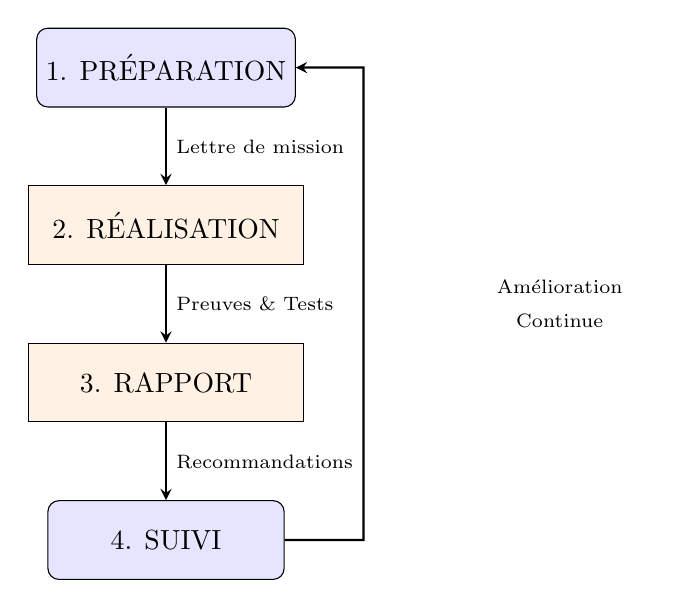
\begin{tikzpicture}[node distance=2cm]
    \tikzstyle{startstop} = [rectangle, rounded corners, minimum width=3cm, minimum height=1cm,text centered, draw=black, fill=blue!10]
    \tikzstyle{process} = [rectangle, minimum width=3.5cm, minimum height=1cm, text centered, draw=black, fill=orange!10]
    \tikzstyle{arrow} = [thick,->,>=stealth]

    \node (p1) [startstop] {1. PRÉPARATION};
    \node (p2) [process, below of=p1] {2. RÉALISATION};
    \node (p3) [process, below of=p2] {3. RAPPORT};
    \node (p4) [startstop, below of=p3] {4. SUIVI};

    \draw [arrow] (p1) -- node[anchor=west] {\scriptsize Lettre de mission} (p2);
    \draw [arrow] (p2) -- node[anchor=west] {\scriptsize Preuves \& Tests} (p3);
    \draw [arrow] (p3) -- node[anchor=west] {\scriptsize Recommandations} (p4);
    
    % Boucle de feedback
    \draw [arrow] (p4.east) -- ++(1,0) -- ++(0,6) -- (p1.east);
    \node at (5,-3) [text width=2.5cm, align=center] {\scriptsize Amélioration Continue};
\end{tikzpicture}
\end{center}
